% Created 2020-04-27 Mon 11:02
% Intended LaTeX compiler: pdflatex
\documentclass[presentation]{beamer}
\usepackage[utf8]{inputenc}
\usepackage[T1]{fontenc}
\usepackage{graphicx}
\usepackage{grffile}
\usepackage{longtable}
\usepackage{wrapfig}
\usepackage{rotating}
\usepackage[normalem]{ulem}
\usepackage{amsmath}
\usepackage{textcomp}
\usepackage{amssymb}
\usepackage{capt-of}
\usepackage{hyperref}
\usetheme{UoB}
\author{Mark Blyth}
\date{\textit{[2020-04-27 Mon]}}
\title{Notes on Gaussian process regression}
\hypersetup{
 pdfauthor={Mark Blyth},
 pdftitle={Notes on Gaussian process regression},
 pdfkeywords={},
 pdfsubject={},
 pdfcreator={Emacs 26.3 (Org mode 9.1.9)}, 
 pdflang={English}}
\begin{document}

\maketitle

\section{Background}
\label{sec:org2f5398a}
\begin{frame}[label={sec:org62c7434}]{Week's goal}
Last week\ldots{}
\begin{itemize}
\item Kernel choice is critical to getting usable results from a GP (moreso than hyperparameters?)
\item Stationary covariance functions aren't able to fully capture neuron dynamics
\item Periodic kernels are harder to fit, but better represent our data
\end{itemize}

This week\ldots{}
\begin{itemize}
\item Decide on a suitable kernel (something non-stationary, non-monotonic)
\item Learn how it works
\item Implement it
\end{itemize}
\end{frame}

\begin{frame}[label={sec:orgaf9099c}]{Week's activities}
\begin{itemize}
\item Read about modelling non-stationarity in GPs
\begin{itemize}
\item Appropriate kernel choice allows us to model non-stationarity
\item There's also more general GPs that allow us to do that
\item These generalised GPs also have other nice features such as heteroscedasticity, and non-Gaussian noise
\end{itemize}
\item Considered experimental issues with GPs
\begin{itemize}
\item Fitting time
\item Noise type
\end{itemize}
\item Wrote up notes about everything I've done with GPs so far
\begin{itemize}
\item Covers some of the key developments in relevant areas of the literature
\end{itemize}
\end{itemize}
\end{frame}

\begin{frame}[label={sec:org191da3b}]{Presentation points}
\begin{enumerate}
\item Highlight what the requirements are for \emph{in silico} experiments
\begin{itemize}
\item Goal: identify what we want from a GP
\end{itemize}
\item Consider how experimental requirements may differ from \emph{in silico}
\begin{itemize}
\item Goal: identify what we want from a GP
\end{itemize}
\item Suggest some possible approaches
\begin{itemize}
\item Goal: find some possible modelling strategies that fit our requirements
\end{itemize}
\item Compare approaches to help decide which approach is best
\begin{itemize}
\item Goal: choose the strategy to work with
\end{itemize}
\end{enumerate}
\end{frame}


\section{GP requirements}
\label{sec:org8ae88c9}
\begin{frame}[label={sec:orgbcf2461}]{Why GPs?}
Always useful to remember why we're doing things!

\vfill

\begin{itemize}
\item All existing CBC methods require us to discretise the system behaviours (outputs, control signals)
\begin{itemize}
\item Neurons spike fast, so this is hard
\end{itemize}
\item Discretisations are necessary in the continuation procedure either to\ldots{}
\begin{itemize}
\item predict and correct the control target,
\item or to iteratively zero the control action
\end{itemize}
\item I'm hoping we can avoid discretisation by using simple transformations of continuous functions, rather than discretised vectors
\end{itemize}

\vfill

This usage case defines our requirements of the Gaussian processes
\end{frame}

\begin{frame}[label={sec:orgeb4d41c}]{The best GP}
The best Gaussian process model satisfies the following:

\vfill

\begin{itemize}
\item Easy to use and understand
\begin{itemize}
\item No need to re-invent the wheel
\item Simplicity is a virtue!
\end{itemize}
\item Gives a \emph{sufficiently} good model
\begin{itemize}
\item Doesn't necessarily have to be perfect, depending on how we use the corrector step
\end{itemize}
\item Easy to train
\begin{itemize}
\item Hyperparameters are either quick and easy to tune, or the model works well even with bad hyperparameters
\end{itemize}
\end{itemize}

\vfill

How simple we can go depends on the data we expect to see
\end{frame}

\begin{frame}[label={sec:org367854f}]{Nice GPs}
A \emph{`nice'} Gaussian process is stationary:

\vfill

\begin{itemize}
\item Strong stationarity: moments (hyperparameters) remain constant across the signal
\item Weak stationarity: mean, variance remain constant across the signal
\item Standard kernels assume stationarity
\item Stationary GP models are analytically tractable, with simple closed-form solutions
\end{itemize}

\vfill
\end{frame}

\begin{frame}[label={sec:org34070bc}]{Practical GPs}
Realistic data aren't stationary; there's two main approaches to handle this:

\vfill

\begin{itemize}
\item Learn a transformation of the data, so that the transformed data are stationary
\item Learn a kernel that can handle the non-stationarity observed in the signal
\end{itemize}

\vfill

Non-stationary models are not always analytically tractable, and require more advanced solution methods.
\end{frame}

\begin{frame}[label={sec:org669b97f}]{Data characteristics for \emph{in silico} CBC}
With computer experiments, we have\ldots{}

\vfill

\begin{itemize}
\item Reliable results with only small amounts of data
\begin{itemize}
\item GP training speed doesn't matter
\end{itemize}
\item Negligable noise
\begin{itemize}
\item Only noise is numerical errors
\end{itemize}
\item `Nice' artificial noise
\begin{itemize}
\item We know exactly what the noise distribution is
\item Noise can be exactly Gaussian
\item Noise can have constant variance
\end{itemize}
\end{itemize}

The only non-standard requirement is that the covariance function must be non-stationary.
\end{frame}

\begin{frame}[label={sec:org3698cd0}]{Data characteristics for \emph{in vitro} CBC}
With real experiments, we have\ldots{}

\vfill

\begin{itemize}
\item Potentially lots of data, if we assume \emph{KHz} sample rates
\begin{itemize}
\item GPs must train quickly
\end{itemize}
\item Unavoidable noise
\begin{itemize}
\item Noise might not be Gaussian, especially for measurement-precision errors
\item Noise variance might change with signal amplitude (eg. multiplicative noise)
\end{itemize}
\end{itemize}
\end{frame}

\begin{frame}[label={sec:org949970f}]{Issues with GPs for \emph{in vitro} CBC}
\begin{itemize}
\item Lots of data
\begin{itemize}
\item GPs are \(\mathcal{O}(n^3)\) to train, so they become impractical with more than a few thousand datapoints
\end{itemize}
\item Non-Gaussian noise
\begin{itemize}
\item GPs are a collection of random variables, whose finite joint distribution is Gaussian
\item This mean GPs only let us model Gaussian noise
\end{itemize}
\item Non-constant signal noise
\begin{itemize}
\item GPs are heteroscedastic -- the noise is assumed to be constant across the signal
\item This might not be true for our experiments
\end{itemize}
\end{itemize}

\vfill

Luckily there's a range of solutions to all these problems!
\end{frame}


\section{Fancy GPs}
\label{sec:org8549c92}
\begin{frame}[label={sec:orga7b3dec}]{Warping GPs}
\begin{itemize}
\item Gaussian proesses assume observations are distributed Gaussian'ly about a true function value
\item When this isn't true, we can try to learn a transformation from the original data to some latent variables, such that the latent variables \emph{are} Gaussian
\item A `nice' GP can then be fitted to the latent variables
\item This allows us to model non-Gaussian noise
\item Only works when it's possible to transform the signal into a stationary GP
\end{itemize}
\end{frame}

\begin{frame}[label={sec:org7612fc3}]{Nonstationary Gaussian processes}
\begin{itemize}
\item Take the standard square-exponential kernel
\item Replace the hyperparameters with latent functions (while retaining PD)
\item Model the latent functions as GPs
\item Design the kernel by fitting those GPs
\item There's clever optimisation techniques, \alert{but they're not necessarily fast, and they require good hyperpriors}
\begin{itemize}
\item Since all neuron data will look similar (in some respects), it's probably possible to train a kernel on a representative dataset; using it on novel data will then only require small optimisations
\end{itemize}
\end{itemize}
\end{frame}

\begin{frame}[plain,label={sec:orgddc51b3}]{Nonstationary GPs work well on biological data}
\begin{center}
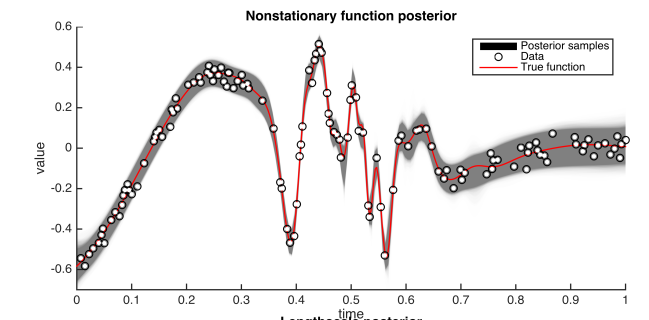
\includegraphics[width=.9\linewidth]{./nonstationary.png}
\end{center}

Source: Heinonen, Markus, et al. "Non-stationary gaussian process regression with hamiltonian monte carlo." Artificial Intelligence and Statistics. 2016.

\vfill

\emph{This also shows how important kernel choice is -- couldn't do that with an SE kernel!}
\end{frame}

\begin{frame}[label={sec:org01a81ff}]{Spectral kernels}
\begin{itemize}
\item Bochner's theorem relates the power spectrum of a signal to its covariance
\item A custom kernel can be designed by fitting a GP to the signal power spectrum, and inverse-Fourier-transforming the result
\begin{itemize}
\item This means we only have to fit one latent GP
\item Derives the kernel directly from the data, so presumably these methods will give the most reasonable kernel for the given problem
\end{itemize}
\item The resulting kernel can model non-monotonic covariance (long-term trends, eg. periodicity), and can be designed to be non-stationary
\item They seem to be exactly the same as the previus non-stationary method, but designed in a perhaps easier-to-compute way
\end{itemize}

\vfill

\begin{itemize}
\item Spectral kernels have also been developed with sparse methods in mind\ldots{}
\end{itemize}
\end{frame}

\begin{frame}[label={sec:org90ef1f1}]{Sparse Gaussian processes}
\begin{itemize}
\item Gaussian processes train in \(\mathcal{O}(n^3)\); this is too slow for \(n>\mathcal{O}(10^3)\) datapoints
\item When faced with big data, we could train a GP by selecting a subset of data to work with
\begin{itemize}
\item This throws away useful information
\end{itemize}
\item Alternative: learn a set of representative latent variables, and train on those
\begin{itemize}
\item For \(m\) latent vars, we get \(\mathcal{O}(nm^2)\) complexity
\end{itemize}
\item Sparse GPs let us train on a smaller number of variables, while minimising loss of information
\begin{itemize}
\item KL divergence gives a measure of the difference between PDFs
\item Variational Bayesian methods give an upper bound on the KL divergence between true posterior, and sparse posterior
\item Gradient descent can then be used to minimise this upper bound
\end{itemize}
\end{itemize}
\end{frame}


\section{The GP choice}
\label{sec:org56758db}
\begin{frame}[label={sec:org41aeab6}]{Choice of GPs}
\begin{itemize}
\item Spectral kernels and the pictured nonstationary GP method will both work well for neuron data
\item The spectral method
\begin{itemize}
\item allows sparsity, so is fast to train
\item provides efficient, easy methods for fitting latent function hyperparameters
\item provides state-of-the-art results
\item has efficient open-source code available, so is easier to use
\end{itemize}
\end{itemize}

That's therefore the method of choice

\vfill

Remes, Sami, Markus Heinonen, and Samuel Kaski. "Neural Non-Stationary Spectral Kernel." arXiv preprint arXiv:1811.10978 (2018).
\end{frame}

\begin{frame}[plain,label={sec:orgc18fcd8}]{}
\begin{center}
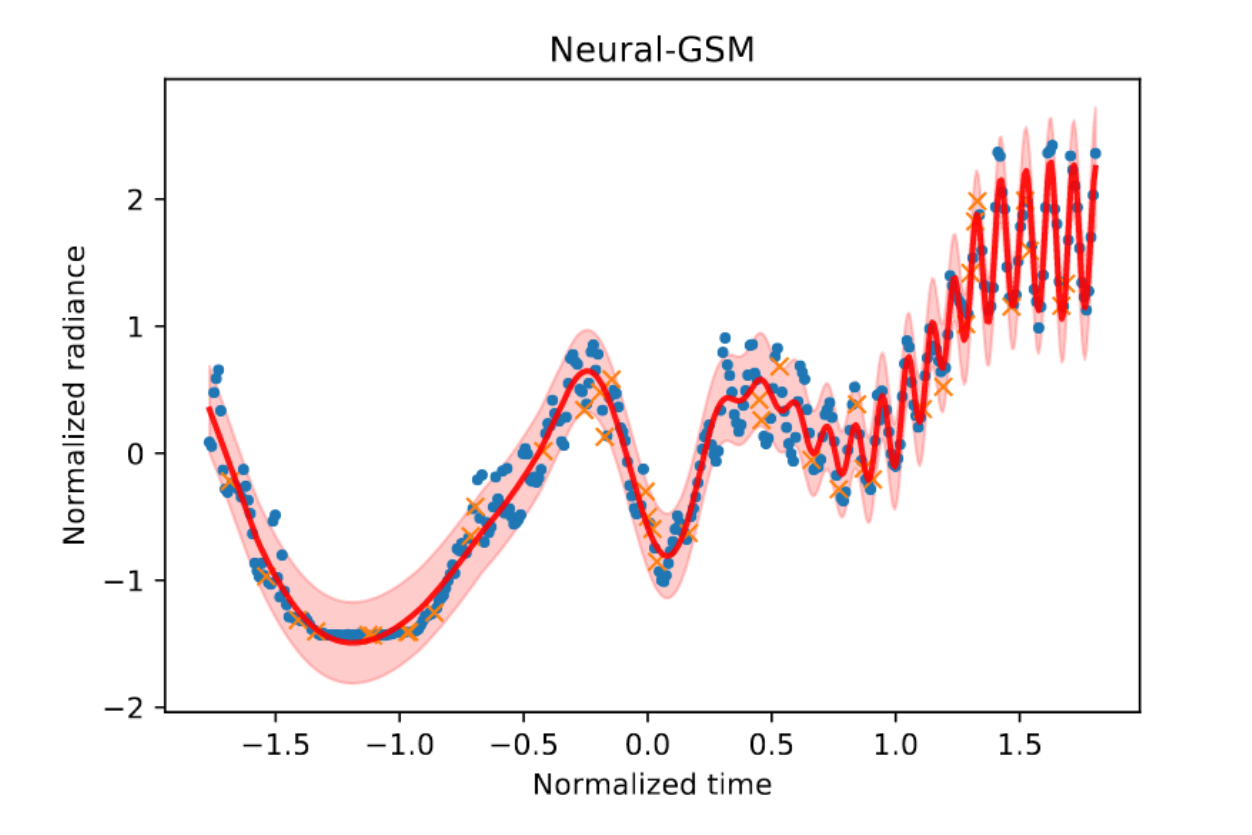
\includegraphics[width=.9\linewidth]{./niceplot.png}
\end{center}
\end{frame}

\section{Next steps}
\label{sec:org096e920}
\begin{frame}[label={sec:orgbb19b69}]{Next steps}
Coursework marking, then\ldots{}

\vfill

\begin{itemize}
\item Days / immediate: Go back and make changes to the continuation paper
\item Week  / medium-term: (Once the paper is finished), find code for, implement, and test the chosen GP scheme
\item Weeks / longer-term: code the predictor-corrector methods, giving a completed CBC code
\end{itemize}
\end{frame}
\end{document}
